Die Meinung von Twitternutzern ist dem Bitcoin--Kurs in Abbildung \ref{fig:result} gegen\"ubergestellt. Die verschiedenen Tweets wurden mit Hilfe der Sentimentanalyse in negative, neutrale und positive Nachrichten unterteilt und in den S\"aulen farblich gekennzeichnet. Die H\"ohe der S\"aulen sentspricht der Anzahl an Nachrichten, die innerhalb eines Zeitintervalls von einer Stunde registriert wurden. Hohe S\"aulen weisen somit auf viele Nachrichten hin, während flache S\"aulen f\"ur wenig Twitter-Meldungen zum Thema Bitcoin stehen. 
Zus\"atzlich ist der Trend des Bitcoin-Kurses aufgetragen. Der jeweilige Wert wurde als Differenz aus Opening- und Closing-Betrag, wie in Abbildung \ref{fig:bitcoin-course} zu sehen, bestimmt. Ein positiver Wert entspricht somit einem steigenden Kursverlauf, ein negativer Wert entsprechend einem fallenden.

\begin{figure}[htb]
	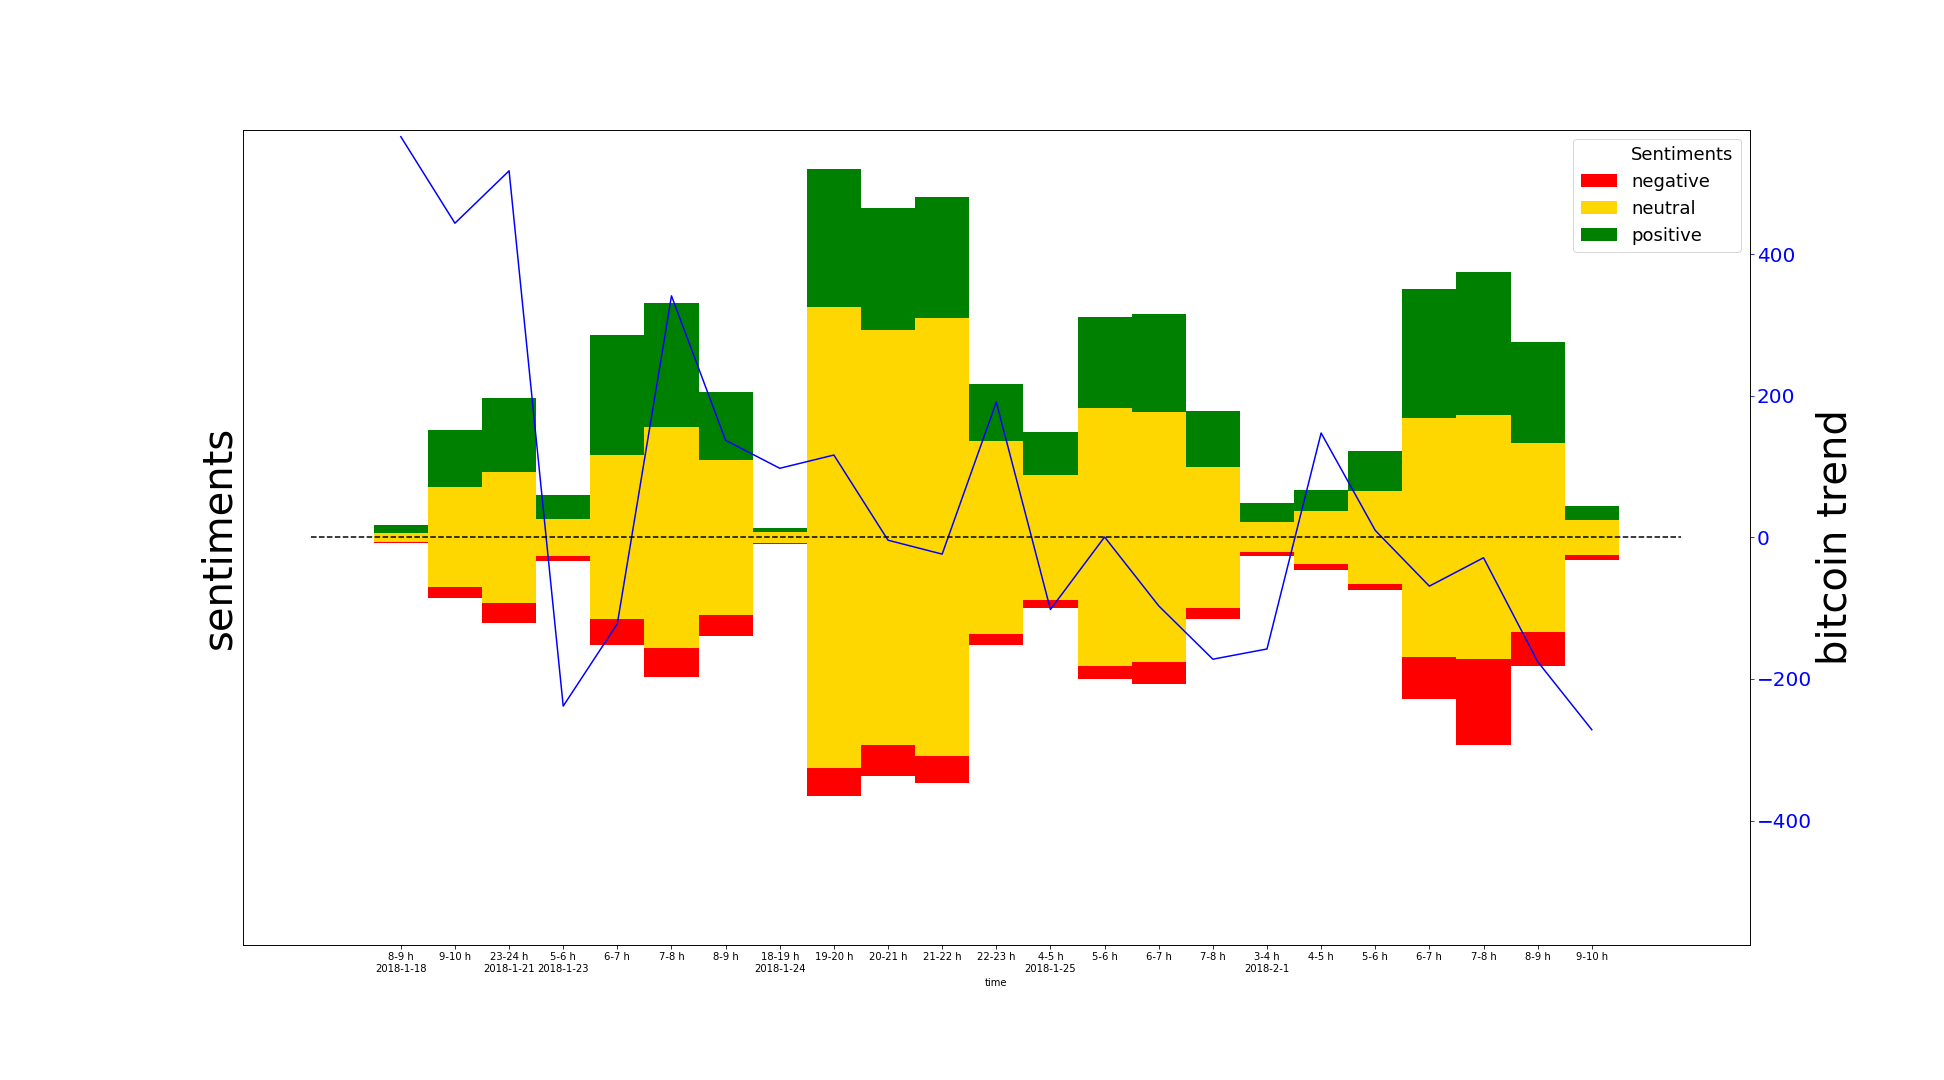
\includegraphics[width=\textwidth]{result}
	\caption{\"Ubersicht der Auswertungsergebnisse. Die blaue Kurve entspricht dem Bitcon-Trend. Die farblich unterteilten S\"aulen stellen die Anzahl an Meinungen dar, die den Clustern positiv (gr\"un), neutral (gelb) und negativ (rot) dar. Die S\"aulenh\"ohe steht f\"ur die Anzahl an Nachrichten pro Stunde.}
	\label{fig:result}
\end{figure}

Es ist zu beachten, dass die dargestellte Zeitachse nicht kontinuierlich verläuft. Viel mehr wurden pro Datum nur Nachrichten aus wenigen Stunden extrahiert. Dieses Verhalten ist auf die Bibliothek \enquote{tweepy\footnote{Siehe http://www.tweepy.org/ .}} zur\"uckzuf\"uhren, mit deren Hilfe die Tweets heruntergeladen wurde. Auf Grund der limitierten Downloadrate bei Twitter und den Einstellungen der Bibliothek wurden Anstelle des gew\"unschten Zeitraums vom 10.01.2018 -- 01.02.2018 lediglich Daten weniger, kurzer Zeitabschnitte heruntergeladen.\\
Aus den vorhandenen Daten lassen sich trotzdem einige Ergebnisse ableiten. 
\begin{itemize}
	\item Wie zu erwarten, ist die Anzahl der Meldungen in den fr\"uhen Morgenstunden geringer als am Abend.
	\item Der Anteil der neutralen Meldungen ist auffallend hoch. 
	\item Es gibt im Allgemeinen mehr positive Tweets zum Thema Bitcoin als negative.
	\item Der Bitcoin-Trend ist am 18.01. und am 21.01.2018 positiv. Zu den jeweiligen Zeitpunkten wurden jedoch nur verh\"altnism\"assig wenig Tweets registriert.
	\item Am 24.01.2018 ist das Interesse am Bitcoin deutlich gestiegen.
	\item Der negative Trend am 01.02.2018 wurde von mehr negativen Tweets begleitet, als zu allen anderen betrachteten Zeitpunkten. Jedoch ist auch die Anzahl der positiven Nachrichten gestiegen.
\end{itemize}

Insgesamt l\"asst sich kein Zusammenhang zwischen den Bitcoin-Trend und den Twitter-Nachrichten erkennen. Dies ist zum einen auf die geringe Stichprobe und die unregelm\"a{\ss}igen Zeitpunkte der Twitterdaten zur\"uckf\"uhren. Zum anderen deuten die vielen, als neutral eingestuften Meldungen darauf hin, dass der von \textit{TextBlob} verwendete Klassifikator nicht ausreichend gut auf die Problemstellung angepasst ist. 



%TODO:  Performance???

%\textcolor{red}{Was ist mit Performance?}